\documentclass[aspectratio=169]{../latex_main/tntbeamer}  % you can pass all options of the beamer class, e.g., 'handout' or 'aspectratio=43'
\usepackage{dsfont}
\usepackage{bm}
\usepackage[english]{babel}
\usepackage[T1]{fontenc}
%\usepackage[utf8]{inputenc}
\usepackage{graphicx}
\graphicspath{ {./figures/} }
\usepackage{algorithm}
\usepackage[ruled,vlined,algo2e,linesnumbered]{algorithm2e}
\usepackage{hyperref}
\usepackage{booktabs}
\usepackage{mathtools}

\usepackage{amsmath,amssymb}

\DeclareMathOperator*{\argmax}{arg\,max}
\DeclareMathOperator*{\argmin}{arg\,min}

\usepackage{pgfplots}
\pgfplotsset{compat=1.16}
\usepackage{tikz}
\usetikzlibrary{trees} 
\usetikzlibrary{shapes.geometric}
\usetikzlibrary{positioning,shapes,shadows,arrows,calc,mindmap}
\usetikzlibrary{positioning,fadings,through}
\usetikzlibrary{decorations.pathreplacing}
\usetikzlibrary{intersections}
\pgfdeclarelayer{background}
\pgfdeclarelayer{foreground}
\pgfsetlayers{background,main,foreground}
\tikzstyle{activity}=[rectangle, draw=black, rounded corners, text centered, text width=8em]
\tikzstyle{data}=[rectangle, draw=black, text centered, text width=8em]
\tikzstyle{myarrow}=[->, thick, draw=black]

% Define the layers to draw the diagram
\pgfdeclarelayer{background}
\pgfdeclarelayer{foreground}
\pgfsetlayers{background,main,foreground}

% Requires XeLaTeX or LuaLaTeX
\usepackage{unicode-math}

\usepackage{fontspec}
%\setsansfont{Arial}
\setsansfont{RotisSansSerifStd}[ 
Path=../latex_main/fonts/,
Extension = .otf,
UprightFont = *-Regular,  % or *-Light
BoldFont = *-ExtraBold,  % or *-Bold
ItalicFont = *-Italic
]
\setmonofont{Cascadia Mono}[
Scale=0.8
]

% scale factor adapted; mathrm font added (Benjamin Spitschan @TNT, 2021-06-01)
%\setmathfont[Scale=1.05]{Libertinus Math}
%\setmathrm[Scale=1.05]{Libertinus Math}

% other available math fonts are (not exhaustive)
% Latin Modern Math
% XITS Math
% Libertinus Math
% Asana Math
% Fira Math
% TeX Gyre Pagella Math
% TeX Gyre Bonum Math
% TeX Gyre Schola Math
% TeX Gyre Termes Math

% Literature References
\newcommand{\lit}[2]{\href{#2}{\footnotesize\color{black!60}[#1]}}

%%% Beamer Customization
%----------------------------------------------------------------------
% (Don't) Show sections in frame header. Options: 'sections', 'sections light', empty
\setbeamertemplate{headline}{empty}

% Add header logo for normal frames
\setheaderimage{
	% 
\includegraphics[height=\logoheight]{figures/TNT_darkv4.pdf}
	
\includegraphics[height=\logoheight]{../latex_main/figures/luh_logo_rgb_0_80_155.pdf}
	% 
\includegraphics[height=\logoheight]{figures/logo_tntluh.pdf}
}

% Header logo for title page
\settitleheaderimage{
	% 
\includegraphics[height=\logoheight]{figures/TNT_darkv4.pdf}
	
\includegraphics[height=\logoheight]{../latex_main/figures/luh_logo_rgb_0_80_155.pdf}
	% 
\includegraphics[height=\logoheight]{figures/logo_tntluh.pdf}
}

% Title page: tntdefault 
\setbeamertemplate{title page}[tntdefault]  % or luhstyle
% Add optional title image here
%\addtitlepageimagedefault{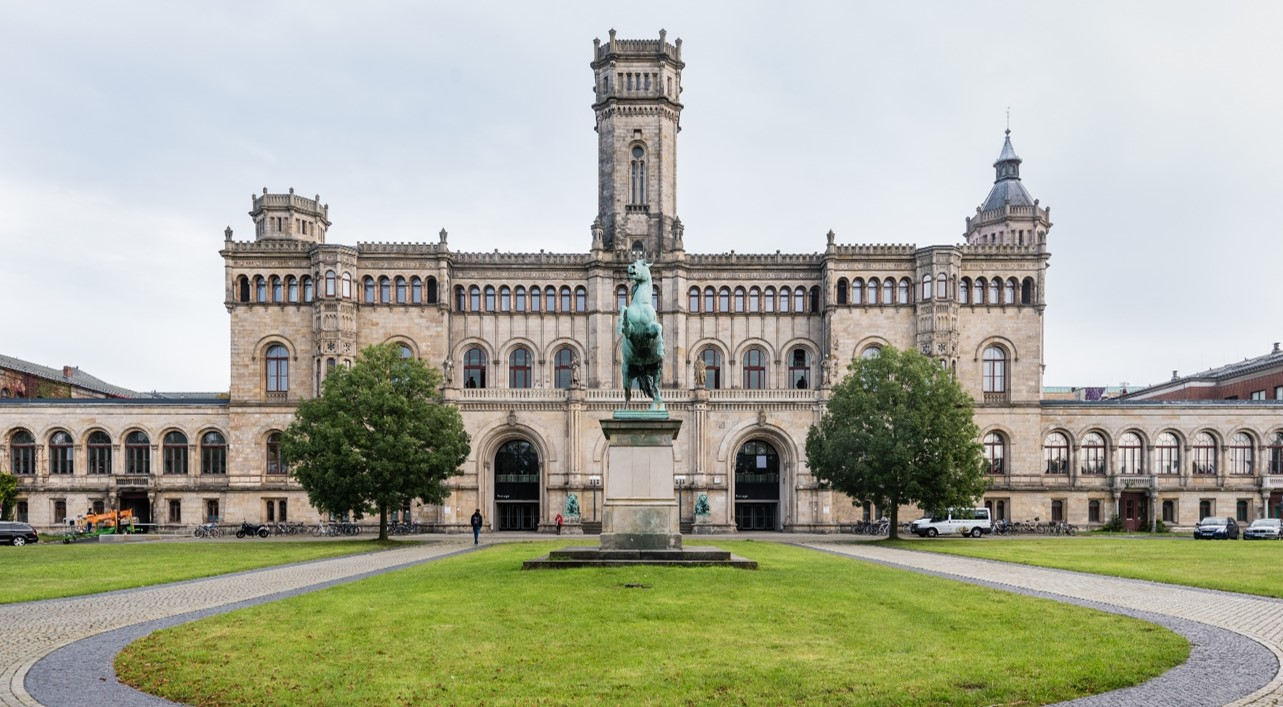
\includegraphics[width=0.65\textwidth]{figures/luh_default_presentation_title_image.jpg}}

% Title page: luhstyle
% \setbeamertemplate{title page}[luhstyle]
% % Add optional title image here
% \addtitlepageimage{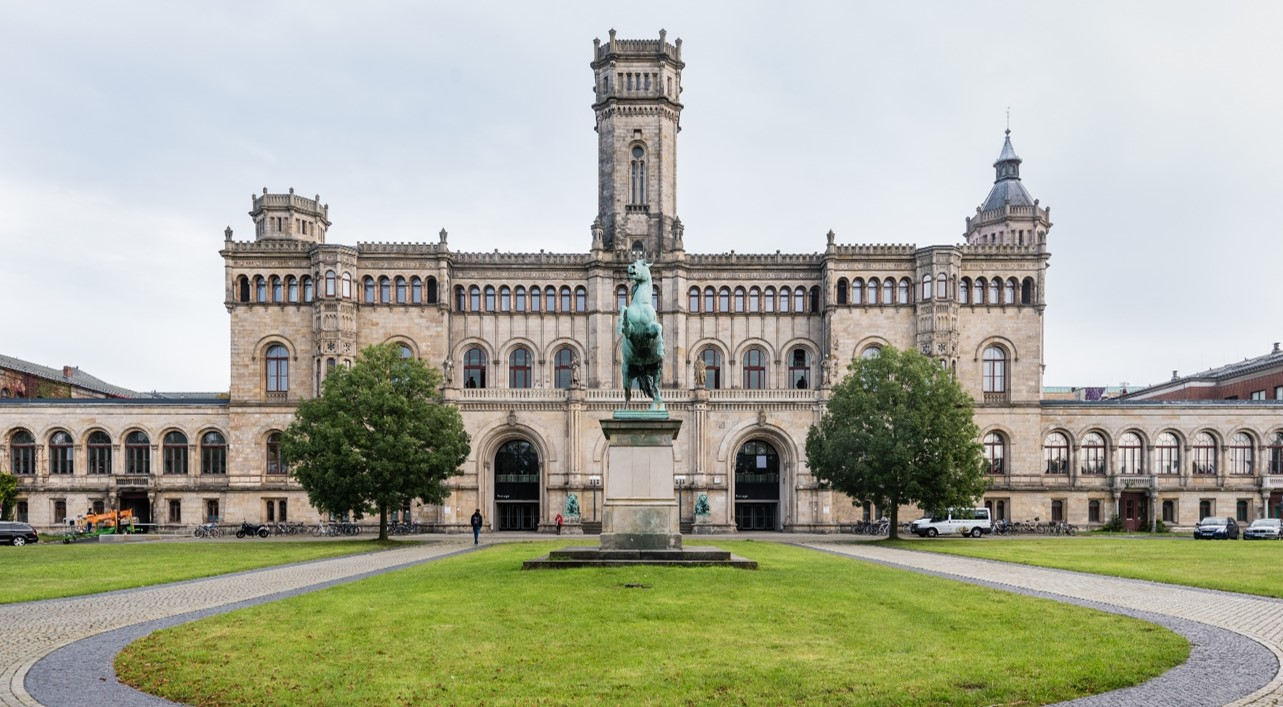
\includegraphics[width=0.75\textwidth]{figures/luh_default_presentation_title_image.jpg}}

\author[Lindauer \& Anand]{Marius Lindauer and Avishek Anand\\[1em]
	
\includegraphics[height=\logoheight]{../latex_main/figures/luh_logo_rgb_0_80_155.pdf}\qquad

\includegraphics[height=\logoheight]{../latex_main/figures/TNT_darkv4}\qquad

\includegraphics[height=\logoheight]{../latex_main/figures/L3S.jpg}	}
\date{Winter Term 2021
}


%%% Custom Packages
%----------------------------------------------------------------------
% Create dummy content
\usepackage{blindtext}

% Adds a frame with the current page layout. Just call \layout inside of a frame.
\usepackage{layout}


\title[Introduction]{iML: Interpretable Models}
\subtitle{Pitfalls and Problems}

%\institute{}


\begin{document}
	
	\maketitle

	%-----------------------------------------------------------------------------------------------------------------------------
    
    \begin{frame}[c]{1. Violating of Assumptions}
    
        \begin{itemize}
            \item Most models have some underlying assumptions
            \begin{itemize}
                \item if there are feature interactions for a linear regression model (e.g., strong correlation),\\ interpreting the weights can be meaningless
                \item[$\leadsto$] there could be many weights explaining the data with the same predictive performance but different explanations
            \end{itemize}
        \end{itemize}
    
    \end{frame}
    
    %-----------------------------------------------------------------------------------------------------------------------------
    
    \begin{frame}[c]{2. Increasing Complexity of Models}
    
        \begin{itemize}
            \item Even interpretable models can become uncomprehensible if too complex;\\
            For example
            \begin{itemize}
                \item complex feature transformations with GAMs
                \item very deep trees
                \item complex ensembles of trees
                \item \ldots
            \end{itemize}
            
        \end{itemize}
    
    \end{frame}
    
    %-----------------------------------------------------------------------------------------------------------------------------
    
        \begin{frame}[c]{3. Full Predictive Pipeline}
    
        \begin{itemize}
            \item Often, we don't only fit a single model to the data at hand
            \item But, we use several pre-processing steps beforehand, for example
            \begin{itemize}
                \item Feature normalization (e.g. standardization)
                \begin{itemize}
                    \item with feature normalization, it gets hard to interpret weights
                    \item without feature normalization, different feature scales might be reflected in your model weights
                \end{itemize}
                \pause
                \item Dimension reduction, e.g., 
                \begin{itemize}
                    \item Interpreting the space of a PCA is hard
                \end{itemize}
                \pause
                \item Feature imputation for missing features
                \begin{itemize}
                    \item Your model might put a lot of weights on imputed features (i.e., never really observed features) 
                \end{itemize}
            \end{itemize}
            
        \end{itemize}
    
    \end{frame}
    
    %-----------------------------------------------------------------------------------------------------------------------------
    
    \begin{frame}[c]{4. Poor Model Fit}
    
        \begin{itemize}
            \item If the model does not fit well the data, there is not point in interpreting the model;\\
            For example
            \begin{itemize}
                \item Decision trees tend to over-fit the data
                \item Linear models often underfit complex data
            \end{itemize}
        \end{itemize}
    
    \end{frame}

	
\end{document}
